\section{Założenia badawcze i konfiguracja eksperymentów}
\label{sec:zalozenia-badawcze-i-konfiguracja-eksperymentow}

Celem części eksperymentalnej pracy jest porównanie skuteczności wybranych modeli rozpoznawania
pisma odręcznego w zadaniu transkrypcji obrazów linii pisma. Szczególny nacisk położono na
próbki pochodzące od osób deklarujących dysgrafię, ponieważ ten typ pisma może istotnie odbiegać
od próbek najczęściej reprezentowanych w publicznych zbiorach danych wykorzystywanych do uczenia
modeli HTR. Analizie poddano modele reprezentujące różne podejścia do rozpoznawania pisma:
Kraken jako klasyczny system HTR pracujący na obrazach linii, TrOCR jako model
enkoder--dekoder oparty na architekturze Transformer oraz Qwen jako multimodalny model językowy
przetwarzający obraz wraz z poleceniem tekstowym.

Eksperymenty zaprojektowano tak, aby oddzielić dwa zagadnienia: jakość modeli w trybie
bez dostosowania do badanego zbioru oraz wpływ dostrajania na wyniki transkrypcji. Z tego powodu
dla każdego modelu przewidziano najpierw ewaluację zero-shot, a następnie wariant po dostrojeniu
na danych treningowych. Porównanie wyników przed i po dostrojeniu pozwala ocenić, czy adaptacja
modelu do konkretnego typu pisma oraz języka poprawia rozpoznawanie, a także czy poprawa ta jest
jednakowa dla próbek niedysgraficznych i dysgraficznych.

W badaniach wykorzystano dwa zbiory danych. Pierwszym z nich jest własny zbiór polskich próbek
pisma odręcznego, opisany szczegółowo w sekcji~\ref{sec:wlasny-zbior-danych}. Zbiór ten obejmuje
2313 zweryfikowanych obrazów linii pochodzących z 320 formularzy. Zawiera próbki osób
deklarujących brak trudności w pisaniu, dysgrafię oraz inne trudności, w tym przede wszystkim
dysleksję. Drugim zbiorem jest malezyjski zbiór \textit{Potential Dysgraphia Handwriting Dataset
of School-Age Children}, zawierający próbki pisma dzieci w dwóch grupach: \textit{Low Potential
Dysgraphia} (LPD) oraz \textit{Potential Dysgraphia} (PD). Oryginalny manifest tego zbioru
zawiera 498 wpisów, natomiast na potrzeby eksperymentów liniowych przygotowano 424 wycinki linii,
analizowane w wariancie surowym oraz w wariancie z automatycznym odwróceniem tonalnym obrazu.

Zastosowanie dwóch zbiorów danych pełni w pracy dwie funkcje. Własny zbiór umożliwia ocenę
modeli na polskim piśmie odręcznym, w tym na znakach diakrytycznych, interpunkcji, liczbach
i krótkich zapisach technicznych. Zbiór malezyjski stanowi natomiast niezależny materiał
porównawczy, który pozwala sprawdzić, czy obserwowane zależności dotyczą wyłącznie przygotowanego
zbioru, czy też pojawiają się również w danych z innego języka i innego sposobu akwizycji.

Podstawową jednostką ewaluacji jest pojedyncza linia pisma. Przyjęcie poziomu linii jest
kompromisem między zbyt małym kontekstem znakowym a zbyt dużą zmiennością całego formularza.
Modele HTR są zwykle trenowane i oceniane właśnie na obrazach linii, ponieważ taki format pozwala
zachować naturalny kontekst sąsiednich znaków i wyrazów, a jednocześnie ogranicza problem
segmentacji strony. W eksperymentach nie stosowano automatycznej korekty językowej po rozpoznaniu.
Wyniki analizowano na podstawie surowych predykcji modeli, aby metryki odzwierciedlały rzeczywistą
zdolność modelu do odczytania pisma, a nie skuteczność późniejszego poprawiania tekstu.

Do oceny jakości transkrypcji wykorzystano metryki CER (\textit{Character Error Rate}) oraz WER
(\textit{Word Error Rate}). CER mierzy względną liczbę operacji edycji na poziomie znaków,
natomiast WER wykonuje analogiczne porównanie na poziomie wyrazów. Metryka CER jest szczególnie
ważna w przypadku pisma dysgraficznego, ponieważ pozwala uchwycić częściowo poprawne rozpoznanie
wyrazu, nawet wtedy gdy cały wyraz zostałby potraktowany przez WER jako błędny. Wyniki raportowano
zarówno zbiorczo, jak i w podziale na grupy trudności, aby nierówny udział poszczególnych grup
w zbiorze nie maskował różnic w jakości rozpoznawania.

\subsection{Scenariusze eksperymentalne (zero-shot vs fine tuning)}
\label{subsec:scenariusze-eksperymentalne}

W pracy przyjęto dwa główne scenariusze eksperymentalne. W scenariuszu zero-shot modele są
uruchamiane bez modyfikacji wag na przygotowanych zbiorach testowych. Taki wariant odpowiada
sytuacji praktycznej, w której gotowy model jest wykorzystywany bez dodatkowego uczenia na danych
pochodzących z konkretnego badania. Wyniki zero-shot stanowią punkt odniesienia dla dalszych
eksperymentów i pozwalają ocenić, jak dobrze modele uogólniają wiedzę wyniesioną z danych
pretreningowych na polskie oraz malezyjskie próbki pisma.

W scenariuszu fine tuning modele są dostrajane z wykorzystaniem części treningowej danego zbioru,
a następnie oceniane na zbiorach walidacyjnym i testowym. Dla własnego zbioru podział wykonano na
poziomie uczestnika, dlatego wszystkie linie jednej osoby znajdują się wyłącznie w jednym splicie.
Ogranicza to ryzyko przecieku stylu pisma między częścią treningową i testową. W przypadku zbioru
malezyjskiego zachowano analogiczną zasadę rozdzielania próbek źródłowych, o ile pozwalały na to
dostępne metadane. Wariant po dostrojeniu umożliwia sprawdzenie, czy modele poprawiają wyniki
po adaptacji do konkretnego zbioru oraz czy dostrojenie na jednym zbiorze wpływa na wyniki
uzyskiwane na drugim zbiorze.

\begin{table}[htbp]
    \centering
    \caption{Plan scenariuszy eksperymentalnych.}
    \label{tab:plan-scenariuszy-eksperymentalnych}
    \begin{tabular}{p{0.18\textwidth}p{0.24\textwidth}p{0.24\textwidth}p{0.23\textwidth}}
        \hline
        Scenariusz & Dane uczące & Dane ewaluacyjne & Cel eksperymentu \\
        \hline
        Zero-shot na zbiorze własnym & Brak dostrajania & Test własnego zbioru polskich formularzy & Ocena gotowego modelu na polskich próbkach pisma, z podziałem na grupy trudności. \\
        Zero-shot na zbiorze malezyjskim & Brak dostrajania & Malezyjski zbiór LPD/PD & Ocena uogólniania modelu na niezależnym zbiorze dotyczącym potencjalnej dysgrafii. \\
        Fine tuning na zbiorze własnym & Część treningowa własnego zbioru & Walidacja i test własnego zbioru oraz zbiór malezyjski & Ocena wpływu adaptacji do polskiego pisma i sprawdzenie przenoszenia efektu na drugi zbiór. \\
        Fine tuning na zbiorze malezyjskim & Część treningowa zbioru malezyjskiego & Walidacja i test zbioru malezyjskiego oraz test własnego zbioru & Ocena adaptacji do danych LPD/PD i wpływu tej adaptacji na polskie próbki formularzowe. \\
        \hline
    \end{tabular}
\end{table}

Wyniki każdego scenariusza analizowano oddzielnie dla poszczególnych modeli. Dodatkowo dla
zbioru własnego raportowano metryki w podziale na grupy: brak trudności, dysgrafia oraz inne
trudności. Dla zbioru malezyjskiego wyniki zestawiano oddzielnie dla grup LPD i PD. Takie
raportowanie jest istotne, ponieważ średnia liczona dla całego zbioru może być zdominowana przez
liczniejszą grupę i nie musi dobrze opisywać jakości rozpoznawania w grupie najważniejszej
z punktu widzenia tematu pracy.

\section{Przygotowanie i przetwarzanie danych}
\label{sec:przygotowanie-i-przetwarzanie-danych}

Przygotowanie danych obejmowało digitalizację formularzy, normalizację geometrii, wycinanie
pojedynczych linii pisma, przypisanie transkrypcji ground truth oraz eksport do formatów
wymaganych przez poszczególne modele. Dla obu zbiorów przyjęto wspólną reprezentację danych:
każda próbka składa się z obrazu linii, tekstu referencyjnego, identyfikatora próbki, informacji
o źródłowym zbiorze oraz etykiety grupy. Ujednolicenie manifestów pozwoliło uruchamiać te same
procedury ewaluacyjne dla modeli Kraken, TrOCR i Qwen.

Własny zbiór formularzy został zapisany w kilku formatach eksportowych. Dla TrOCR przygotowano
pliki CSV zawierające ścieżki do obrazów i transkrypcje referencyjne. Dla Qwen utworzono pliki
JSONL, w których każda próbka zawiera obraz, polecenie transkrypcji i oczekiwaną odpowiedź. Dla
Kraken przygotowano pary plików graficznych i tekstowych zgodne z konwencją \texttt{.png} oraz
\texttt{.gt.txt}. Niezależnie od formatu eksportu zachowano te same identyfikatory próbek,
co umożliwia porównywanie wyników między modelami na dokładnie tych samych liniach.

Transkrypcję ground truth przygotowywano zgodnie z zasadą możliwie wiernego odczytu tego, co
zostało zapisane przez uczestnika. Nie poprawiano automatycznie błędów ortograficznych,
interpunkcyjnych ani brakujących znaków diakrytycznych, jeżeli wynikały one z zapisu na formularzu.
Jeżeli odczyt był niejednoznaczny, próbkę oznaczano statusem \textit{niepewne}; jeżeli wycinek
nie nadawał się do rzetelnej oceny, otrzymywał status \textit{wyklucz}. Do głównego eksportu
i ewaluacji trafiały wyłącznie próbki o statusie \textit{OK}. Dzięki temu metryki CER i WER nie
są obciążone arbitralnymi decyzjami w przypadkach, w których nawet ręczna interpretacja zapisu
nie była jednoznaczna.

Do usprawnienia walidacji przygotowano lokalny program przeglądarkowy. Aplikacja wyświetlała
obraz całego formularza, wycięte linie pisma, metadane uczestnika oraz przypisany ground truth.
Zmiana wartości w interfejsie była zapisywana bezpośrednio w plikach CSV, na podstawie których
następnie przebudowywano eksporty dla poszczególnych modeli. Widok programu wykorzystanego do
walidacji i uzupełniania transkrypcji przedstawiono na rysunku~\ref{fig:panel-walidacji-gt}.

\begin{figure}[htbp]
    \centering
    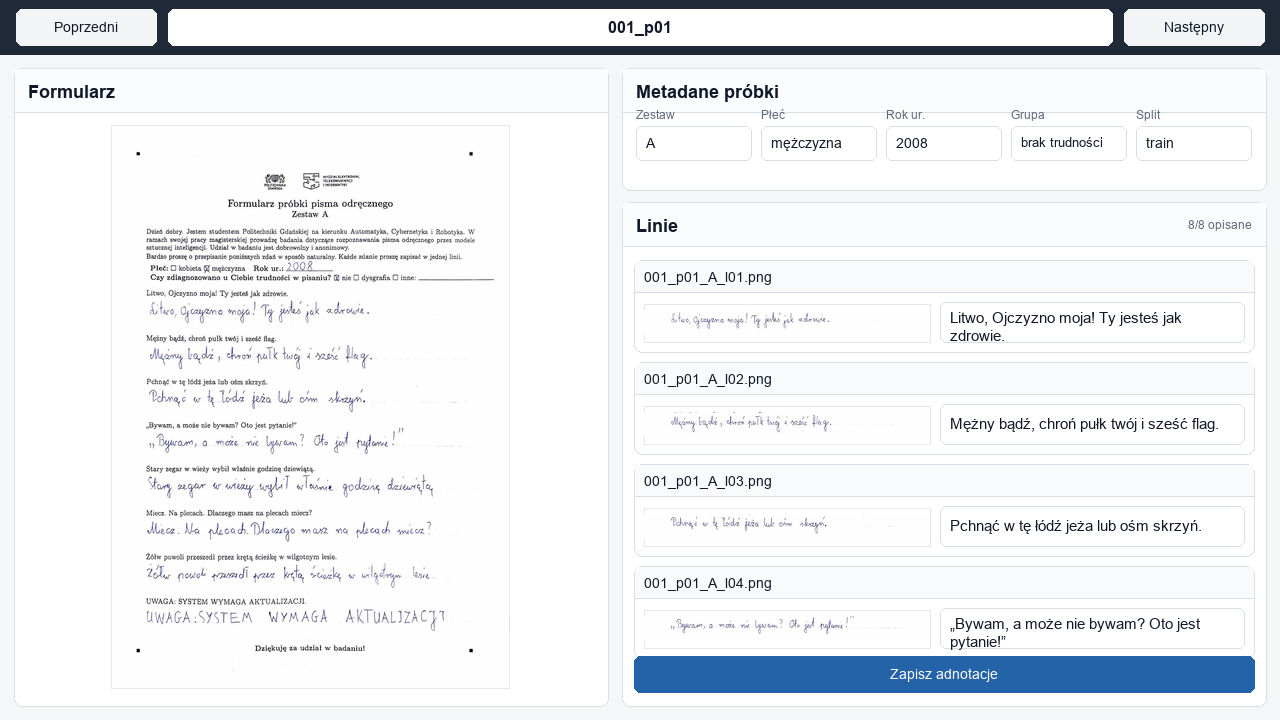
\includegraphics[width=0.95\textwidth]{Formularze/processed_320_check/stats_thesis/figures/panel_walidacji_gt.png}
    \caption{Panel programu wykorzystanego do walidacji metadanych i transkrypcji ground truth.}
    \label{fig:panel-walidacji-gt}
\end{figure}

\subsection{Preprocessing}
\label{subsec:preprocessing}

Preprocessing własnych formularzy rozpoczynał się od konwersji plików PDF lub obrazów wejściowych
do postaci rastrowej. Następnie wykrywano czarne znaczniki narożne umieszczone na formularzu.
Ich położenie umożliwiało wyznaczenie transformacji perspektywicznej i sprowadzenie każdego
arkusza do wspólnego układu współrzędnych. Dzięki temu dalsze operacje, takie jak odczyt pól
metadanych i wycinanie linii pisma, mogły być wykonywane na stałych obszarach formularza.

Po normalizacji geometrycznej wycinano pola odpowiadające płci, rokowi urodzenia, deklarowanym
trudnościom w pisaniu oraz ośmiu liniom przeznaczonym na odpowiedzi. Pola wyboru analizowano
na podstawie gęstości ciemnych pikseli, co pozwalało automatycznie zasugerować zaznaczoną płeć
i deklarowaną trudność. Rok urodzenia odczytywano półautomatycznie z użyciem modelu Qwen,
a następnie weryfikowano ręcznie w panelu walidacyjnym. Taki tryb pracy znacząco ograniczył
liczbę wartości przepisywanych ręcznie, jednocześnie pozostawiając człowiekowi kontrolę nad
ostatecznym zapisem metadanych.

Wycinki linii były przygotowywane tak, aby zawierały przede wszystkim pismo odręczne uczestnika.
Ponieważ na formularzu znajdowały się również wydrukowane zdania referencyjne i linie pomocnicze,
zastosowano procedurę wybielania elementów drukowanych na podstawie szablonu pustego formularza.
Dla nietypowych przypadków, w których uczestnik zapisał odpowiedź w dwóch wierszach albo znacznie
wyszedł poza linię, dopuszczono rozszerzone wycinki obejmujące większy obszar pionowy. Takie
próbki nie były automatycznie odrzucane, ponieważ właśnie w przypadku pisma dysgraficznego
niestandardowe rozmieszczenie tekstu jest częścią obserwowanego zjawiska. Decyzję o pozostawieniu
albo wykluczeniu próbki podejmowano podczas ręcznej walidacji.

Preprocessing zbioru malezyjskiego miał inny charakter, ponieważ dane pochodziły z gotowego
zbioru zewnętrznego. Oryginalny plik CSV zawierał ścieżkę do obrazu, tekst referencyjny, grupę
LPD albo PD oraz identyfikator tekstu. Na potrzeby porównania z własnym zbiorem przygotowano
manifest liniowy, w którym dłuższe zapisy zostały rozdzielone na pojedyncze linie. Dla każdej
linii zapisano transkrypcję odpowiadającą widocznemu fragmentowi tekstu. Dodatkowo przygotowano
wariant z automatycznym odwróceniem tonalnym obrazu, ponieważ część modeli uzyskuje stabilniejsze
wyniki, gdy tło i kolor pisma są zgodne z rozkładem danych, na których model był pierwotnie
trenowany.

W obu zbiorach zachowano rozdzielenie danych treningowych, walidacyjnych i testowych na poziomie
osoby lub źródłowego obrazu, o ile pozwalały na to metadane. Celem takiego podziału było uniknięcie
sytuacji, w której model uczy się charakterystycznego stylu pisma danej osoby na jednej próbce,
a następnie jest oceniany na innej linii tej samej osoby. Po zakończeniu preprocessingu wszystkie
eksporty zostały sprawdzone pod względem liczby obrazów, liczby transkrypcji oraz zgodności
identyfikatorów między formatami.

\section{Środowisko implementacyjne}
\label{sec:srodowisko-implementacyjne}

Implementację przygotowano w środowisku Python uruchamianym lokalnie na systemie Windows.
Do przetwarzania formularzy wykorzystano biblioteki OpenCV, PyMuPDF, Pillow i pandas. OpenCV
służyło do wykrywania znaczników, progowania obrazów, transformacji perspektywicznej oraz operacji
morfologicznych. PyMuPDF wykorzystywano do rasteryzacji plików PDF, Pillow do operacji na obrazach,
a pandas do obsługi manifestów CSV i kontroli spójności metadanych. Statystyki zbioru oraz wykresy
przygotowano z użyciem bibliotek pandas i matplotlib, a zestawienia tabelaryczne eksportowano
również do plików XLSX.

Eksperymenty z modelami rozpoznawania pisma realizowano z użyciem bibliotek PyTorch,
Transformers oraz Kraken. Modele TrOCR i Qwen uruchamiano przez interfejs biblioteki
Transformers, natomiast model Kraken przez narzędzia i klasy udostępniane przez pakiet Kraken.
Skrypty ewaluacyjne zapisywały predykcje modeli, wartości metryk CER i WER, czas inferencji oraz
podstawowe informacje o konfiguracji uruchomienia. Dzięki temu każdy wynik można powiązać
z modelem, zbiorem danych, wariantem preprocessingu i konkretną próbką wejściową.

Cały proces przygotowania danych został oparty na jawnych manifestach. Pełny manifest zawiera
również próbki oznaczone jako niepewne i wykluczone, natomiast manifesty eksportowe zawierają
wyłącznie próbki przeznaczone do głównej ewaluacji. Takie rozdzielenie ułatwia odtworzenie procesu
decyzyjnego i pozwala w razie potrzeby wrócić do odrzuconych przypadków bez utraty informacji
o ich pochodzeniu. Dodatkowo lokalny panel walidacyjny umożliwiał szybkie poprawianie metadanych
i transkrypcji, po czym eksporty dla Kraken, TrOCR i Qwen mogły zostać przebudowane na podstawie
aktualnej wersji plików CSV.

Wyniki eksperymentów zapisywano w postaci plików CSV, JSON, JSONL i XLSX. Taki format ułatwia
zarówno automatyczne liczenie metryk, jak i późniejsze tworzenie tabel oraz wykresów do pracy.
Istotnym elementem środowiska była powtarzalność przetwarzania: te same manifesty źródłowe były
wykorzystywane przez wszystkie modele, a podział danych na część treningową, walidacyjną i testową
był przechowywany razem z metadanymi próbek. Dzięki temu różnice w wynikach można interpretować
jako efekt działania modeli i wariantów preprocessingu, a nie jako skutek przypadkowo odmiennego
doboru danych wejściowych.
